 \documentclass[
	% -- opções da classe memoir --
	12pt,				% tamanho da fonte
	openright,			% capítulos começam em pág ímpar (insere página vazia caso preciso)
	oneside,			% para impressão em verso e anverso. Oposto a oneside
	a4paper,			% tamanho do papel. 
	% -- opções da classe abntex2 --
	chapter=TITLE,		% títulos de capítulos convertidos em letras maiúsculas
	section=TITLE,		% títulos de seções convertidos em letras maiúsculas
	subsection=TITLE,	% títulos de subseções convertidos em letras maiúsculas
	%subsubsection=TITLE,% títulos de subsubseções convertidos em letras maiúsculas
	% -- opções do pacote babel -
	french,				% idioma adicional para hifenização
	spanish,			% idioma adicional para hifenização
	english,			% o último idioma é o principal do documento
	brazil
	]{abntex2}
	
%----------------------------------------------------------------
% Pacotes fundamentais
%----------------------------------------------------------------
	
%\usepackage[top=2.5cm, 
%			bottom=2.5cm, 
%			left=2.5cm, 
%			right=2.5cm]{geometry} %definir margem	
\usepackage{indentfirst}		% Indenta o primeiro parágrafo de cada seção.
\usepackage{graphicx}			% Inclusão de gráficos


\usepackage[affil-it]{authblk}
\usepackage{caption} %Customization of appearance and placement of captions for figures,etc.
\usepackage{placeins}
\usepackage{subcaption}%multiple floats (figures, tables) within one environment
\usepackage{booktabs}%melhora tabelas
\usepackage{enumerate}%criar items e subitem

\usepackage{amssymb,amsthm,amsmath,amsfonts} %simbolos matematicos
\usepackage{pgfplots}

\usepackage[brazilian,hyperpageref]{backref}	 % Paginas com as citações na bibl
\usepackage[num]{abntex2cite}	% Citações padrão ABNT

\usepackage{float}


%----------------------------------------------------------------
%pacotes para usar acentos
%----------------------------------------------------------------
\usepackage[utf8]{inputenc}
\usepackage[T1]{fontenc}
\usepackage{lmodern}

% ---------------------------------------------------------------
% Pacotes de citações
% ---------------------------------------------------------------
\usepackage[brazilian,hyperpageref]{backref}	 % Paginas com as citações na bibl
\usepackage[num]{abntex2cite}	% Citações padrão ABNT



\interfootnotelinepenalty=10000

% ---------------------------------------------------------------
% Espaçamentos entre linhas e parágrafos 
% ---------------------------------------------------------------

% O tamanho do parágrafo é dado por:
\setlength{\parindent}{1.3cm}

% Controle do espaçamento entre um parágrafo e outro:
\setlength{\parskip}{0.2cm}  % tente também \onelineskip




%----------------------------------------------------------------
\providecommand{\sin}{} \renewcommand{\sin}{\hspace{2pt}\mathrm{sen}}		% Redefine a escrita do seno
\providecommand{\tan}{} \renewcommand{\tan}{\hspace{2pt}\mathrm{tg}}		% Redefine a escrita da tangente
\providecommand{\cos}{} \renewcommand{\cos}{\hspace{2pt}\mathrm{cos}}		% Redefine a escrita da tangente




% ---
% compila o indice
% ---
\makeindex


%-------------------------------
% Início do documento
\begin{document}

\begin{capa}

\newcommand{\HRule}{\rule{\linewidth}{0.5mm}} %comando para as linhas horizontais

%----------------------------------------------------------------------------------------
%	HEADING SECTIONS
%----------------------------------------------------------------------------------------

\centering % Center everything on the page
\vspace{-2cm}
\textsc{\LARGE Universidade Federal de Santa Catarina}\\[0.5cm] 
\textsc{\large Centro Tecnológico}\\ % department
\textsc{\large Programa de Pós-Graduação em Engenharia Mecânica}\\[4cm] % department

%----------------------------------------------------------------------------------------
%	TITLE SECTION
%----------------------------------------------------------------------------------------
	
\HRule \\[1cm]
{ \huge \bfseries Aeroacústica Computacional   }\\[1.5cm] % Title of the document
{ \huge \bfseries Trabalho 1 }\\[1cm] 
\HRule \\[6cm]
	
	 
%----------------------------------------------------------------------------------------
%	AUTHOR SECTION
%----------------------------------------------------------------------------------------
	\begin{flushleft}
	\Large Aluno: Anderson Bringhenti \\[0.5cm]
	\Large Professor: Andrey R. da Silva
	\end{flushleft}
%----------------------------------------------------------------------------------------
%	DATE SECTION
%----------------------------------------------------------------------------------------
	\vspace{2cm}
	{\large Florianópolis, Brasil - \today} % Date, change the \today to a set date if you want to be precise
	\vfill % Fill the rest of the page with whitespace
\end{capa}





\tableofcontents



%-----------------------
\chapter{Introdução}
\label{sec:introd}
O presente trabalho é comparar os resultados numéricos e analíticos para a propagação de uma onda cilíndrica bidimensional. O modelo numérico empregado é o LBGK(D2Q9), no qual a sua implementação numérica foi fornecida. Para a comparação os resultado numéricos foram obtidos através da solução da equação da onda viscosa, dada por:
 %%%%%%%%%%%%%%%%%%%%%%%%%%%%%%%%
\begin{equation}
\left( 1-\frac{2\nu}{c_{o}^2}\partial_{t}\right)\nabla^2p=\frac{1}{c_{p}^2}\partial_{t}^2 p,
\label{eq:wave}
\end{equation}
%%%%%%%%%%%%%%%%%%%%%%%%%%%%%%%%
onde $\nu$ e $c_o$ são as viscosidade cinemática e a velocidade do som no meio, respetivamente.

 Para uma onda cilíndrica propagante, a solução exata estacionária da Equação \ref{eq:wave}, é dada por:
%%%%%%%%%%%%%%
\begin{equation}
p~5=AH_{o}^{(2)}kr e^{j \omega t},
\label{eq:solution}
\end{equation}
%%%%%%%%%%%%%%%%%%%%
onde $A$ é a amplitude da onda, $H_{o}^{(2)}$ é a função de Hankel do segundo tipo e ordem 0, e $r$ é a distância radial, a partir fonte sonora. $k=\frac{\omega}{c_p}-j\alpha$ é o número de onda complexo e $\alpha$ é o coeficiente de absorção espacial, expresso por:
%%%%%%%%%%%%%%
\begin{equation}
\alpha=\frac{\omega}{c_p \sqrt{2}}\sqrt{\frac{\sqrt{1+(\omega \tau_{s})^2}-1}{1+(\omega \tau_{s})^2}},
\label{eq:alpha}
\end{equation}
%%%%%%%%%%%%%%%%%%%%
sendo que a implementação da Equação \ref{eq:solution} também foi fornecida.

%%%%%%%%%%%%%%%%%%
\chapter{Desenvolvimento}
\label{sec:des}

\section{Número de incrementos de tempo}
\label{sec:B1}

A primeira tarefa no desenvolvimento deste trabalho foi encontrar o número de passos de tempo necessários (NTS) para uma perturbação propagar do centro até as extremidades. Como o código fornecido não leva em consideração nenhuma condição de contorno específica em sua fronteira, o resultado após este momento não possui informações. A Equação \ref{eq:NTS} mostra a forma que foi calculado o número de incrementos necessários. 
\begin{equation}
NTS = \frac{M_c}{2} \frac{1}{c_{lat}}.
\label{eq:NTS}
\end{equation} 
onde $M_c$ é o número de blocos até a extremidade e $c_{lat}$ é a velocidade do som em unidades de Lattice. Para o caso utilizado $M_c = 300$ e $c_{lat} = 1/\sqrt{3}$ assim
\begin{equation*}
NTS = 150\sqrt{3}
\label{eq:NTS}
\end{equation*} 

\section{Fonte harmônica}
\label{sec:B2}

Uma fonte acústica harmônica foi criado no centro do domínio computacional através da imposição de uma flutuação de densidade harmônica, dada por
%%%%%%%%%%%%%%
\begin{equation}
\rho(x,ta\Delta t)=\rho_o+A sin(2\pi f(ta-1)\Delta t),
\label{eq:fonte}
\end{equation}
%%%%%%%%%%%%%%%%%%%%
onde $f$ é a frequência, $ta$ é o incremento de tempo computacional, $\Delta t$ o incremento de tempo e $A=0,001$ a amplitude da perturbação de densidade da fonte. A frequência da fonte é dada por
%%%%%%%%%%%%%%
\begin{equation}
f=\frac{c_{\text{L}}}{n\Delta x},
\label{eq:freq}
\end{equation}
%%%%%%%%%%%%%%%%%%%%
onde n é o número de células por comprimento de onda. Assim, a cada incremento de tempo $ta$ a densidade no centro da malha é recalculada de forma a incluir o termo fonte.

A Figura \ref{fig:font_harm} contém o campo acústico resultante no final da propagação para $n=8$. 
\begin{figure}[H]
\centering
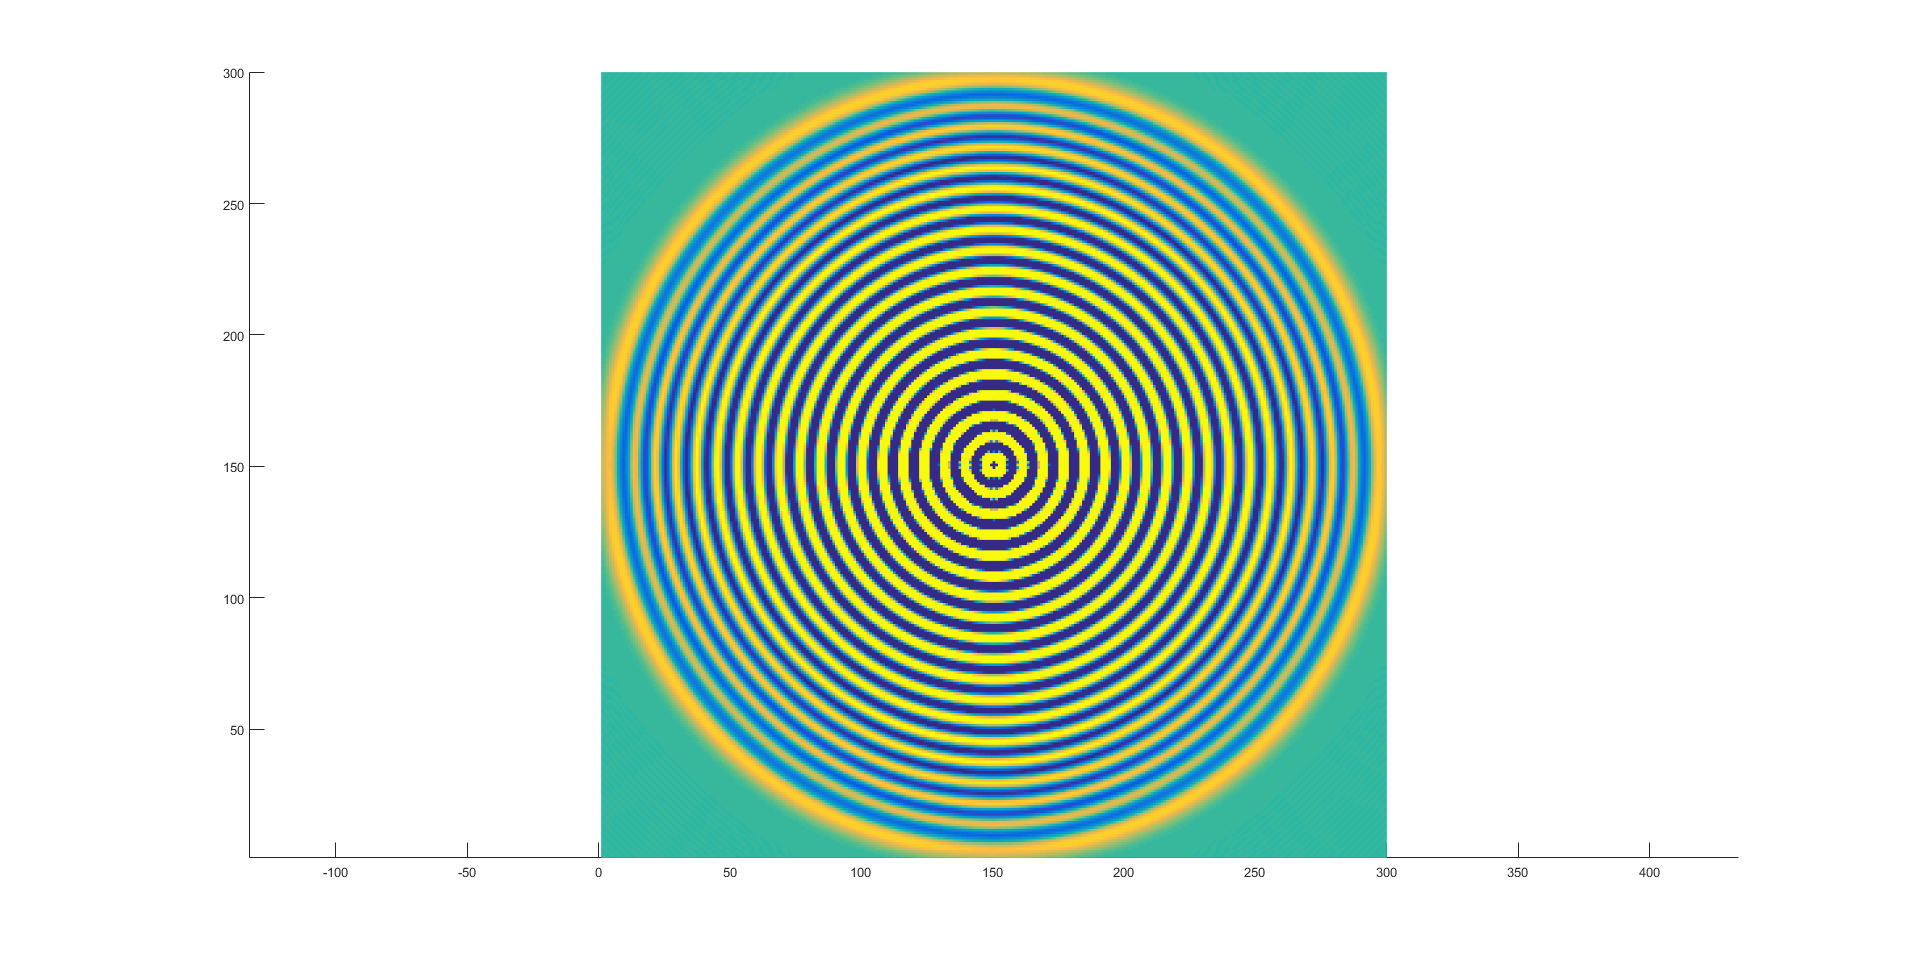
\includegraphics[width=0.8\linewidth]{fonteharm}
\caption{Propagação acústica devido a uma perturbação harmônica.}
\label{fig:font_harm}
\end{figure}

\section{Efeito da discretização da malha}
\label{sec:B3}

Com o modelo numérico configurado, a flutuação de pressão é obtida para $ta=NTS$, ao longo do vetor de coordenadas de lattice, $x=[150:300,150]$, após é comparada a solução numérica com a solução analítica para três diferentes discretizações do comprimento de onda ($n=8, 16$ e $25$ células por comprimento de onda). Como a velocidade do som é dada por $c = \lambda f$ e o comprimento de onda discretizado por $ \lambda = d \Delta x$, a frequência da fonte em $Hz$ será então
\begin{equation*}
f = \frac{c}{d \Delta x},
\end{equation*}
e que estão listadas na Tabela \ref{tab:discreitzacao}.
%%%%%%%%%%%%%%%
\begin{table}[htb!]
\centering
\caption{Frequência da fonte para diferentes números de pontos por comprimento de onda.}%
\label{tab:discreitzacao}
\begin{tabular}{cc}
\toprule
Número de pontos por comprimento de onda & Frequência da fonte [Hz] \\
\midrule
8 & 25500 \\
\midrule
16 & 12750 \\
\midrule
25 & 8160 \\
\bottomrule
\end{tabular} 
\end{table}

Como o método LBGK é adimensional, é preciso fazer a conversão para unidades físicas, de forma a permitir a comparação com o resultado analítico. A relação entre a pressão em lattice e real está disponível em, \citeauthoronline{Viggen2014},\citeyear{Viggen2014}, é dada por:
\begin{equation}
p_{ph} = C_p\left(\frac{c_{0,ph}}{c_{0,la}}\right)^{2}p_{la}
\end{equation}
onde $c_p = \frac{\rho_{ph}}{\rho_{la}}$, ou seja, a razão entre a densidade média física e a densidade média em lattice. 
A Figura \ref{fig:convergencia} mostra o comparativo entre o resultado analítico e numérico para as três diferentes discretização.
%%%%%%
\begin{figure}[H]
\centering
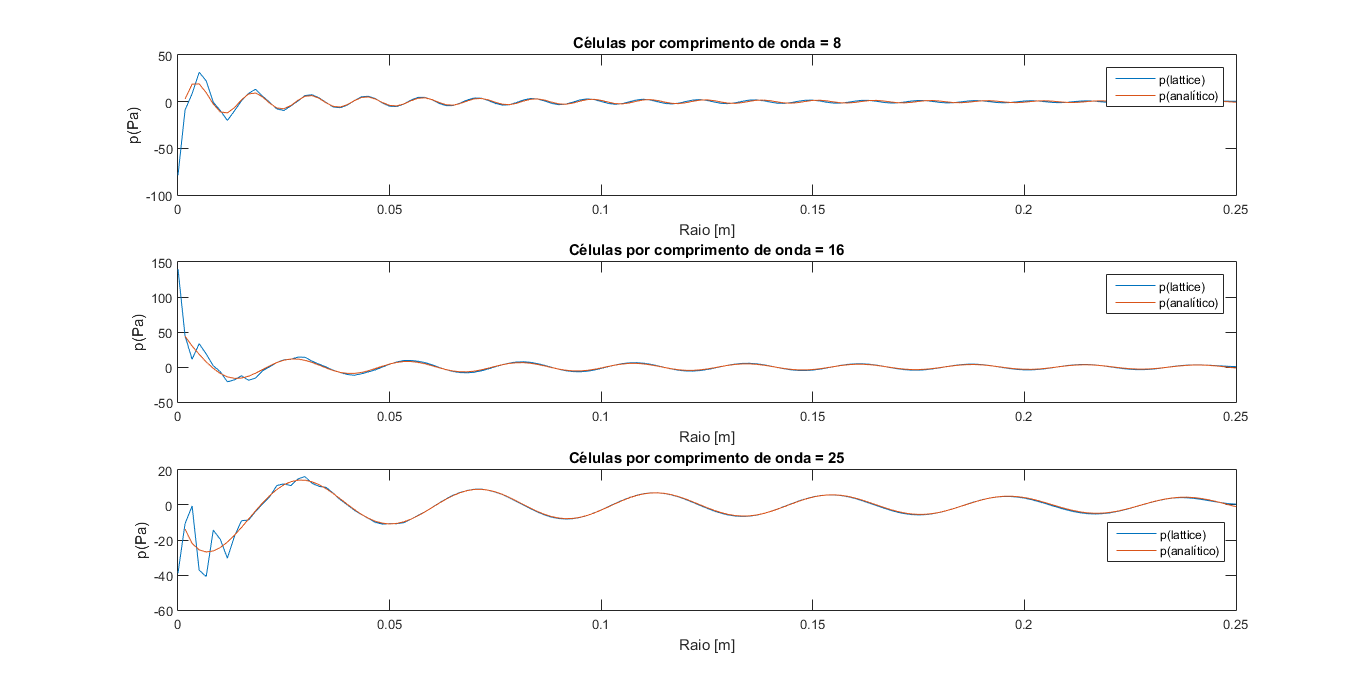
\includegraphics[width=1\textwidth]{conv.png}
\caption{Comparação de resultados numéricos e analíticos da flutuação de pressão para $n=8$, $n=16$ e $n=25$.}
\label{fig:convergencia}
\end{figure}
%%%%%%%%%

\section{Efeito da diferença na viscosidade}
\label{sec:B3}

O modelo LBGK calcula a viscosidade cinemática física com base na viscosidade cinemática adimensional. Como visto no início, a primeira pode ser calculada por
\begin{equation}
\nu_p = \nu \frac{\Delta x^2}{\Delta t}.
\end{equation}

Neste caso, resulta em aproximadamente $\nu = 8,8 \times 10^{-3}$ m\textsuperscript{2}/s. A viscosidade cinemática do ar, na CNTP, é de aproximadamente $\nu = 1,5 \times 10^{-5}$ m\textsuperscript{2}/s, indicando uma diferença de $O(2)$ entre estes dois valores. A comparação entre estes no resultado analítico está na Figura \ref{fig:visc}.

\begin{figure}[H]
\centering
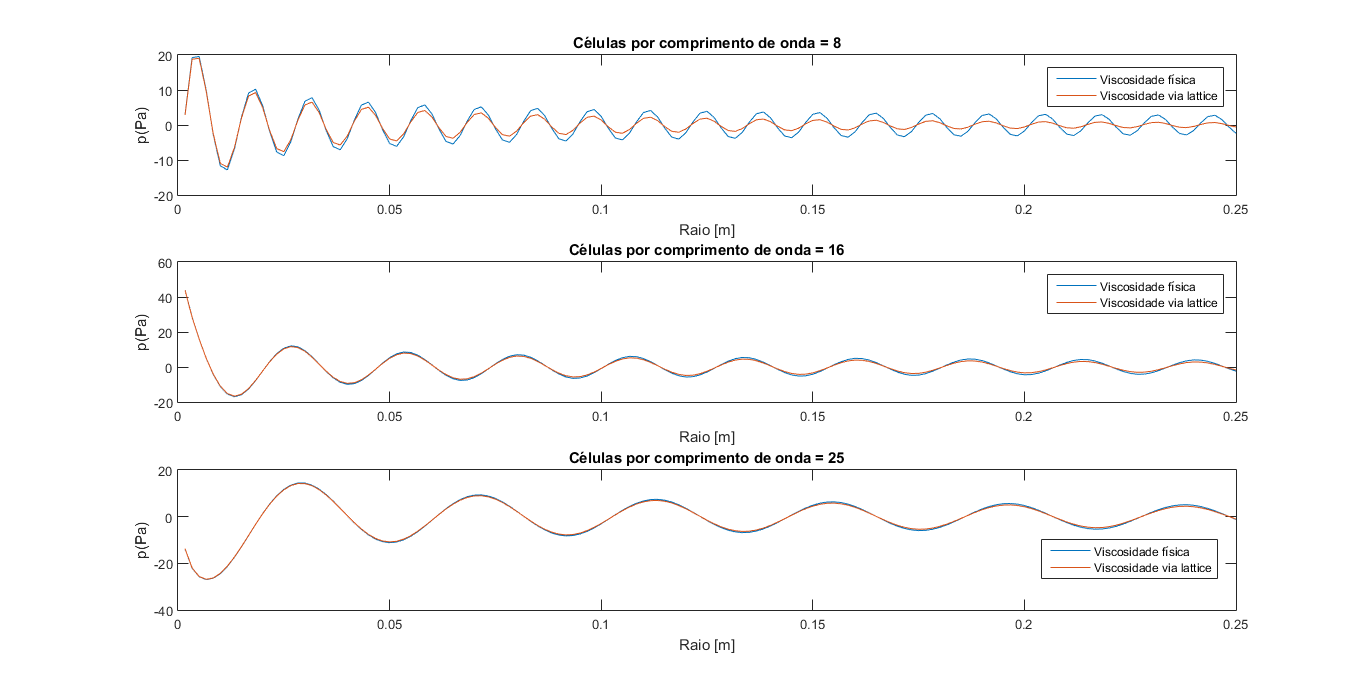
\includegraphics[width=1\linewidth]{visc.png}
\caption{Comparação entre os resultados utilizado a viscosidade real e a viscosidade obtida via lattice.}
\label{fig:visc}
\end{figure}
%%%%%%%%%

\chapter{Considerações Finais}
\label{sec:consideracoes}

\begin{itemize}

\item Os resultados numérico e analítico possuem uma maior discrepância para o caso menos discretizado ($d=8)$. Segundo \citeauthoronline{Wilde2006},\citeyear{Wilde2006}, deve-se haver mais de 12 pontos por comprimento de onda para que não haja erros na fase e na amplitude.

\item Para altas discretizações $(n=16, 25)$, uma diferença de resultados é visualizada próximo a fronteira do número de células analisadas. Segundo \citeauthoronline{Viggen2010},\citeyear{Viggen2010}, esses picos não são erros e estão atribuídos a um decaimento transiente que ocorre em torno da primeira frente de onda, a qual se propaga até o final da análise.

\item A diferença entre a viscosidade física calculada via LBGK e o valor de tabela de propriedade de fluido é de $O(2)$, porém isto não provoca erros significativos nos resultados, como demonstrado na Figura \ref{fig:visc}. A viscosidade física é usada no modelo analítico para calcular
\begin{equation*}
\tau_s = \frac{2 \nu}{c_s^2}.
\end{equation*}
O termo $\tau_s$ é usado no cálculo do coeficiente de absorção através de
\begin{equation*}
\alpha = \frac{\omega}{c_s \sqrt{2}} \sqrt{\frac{\sqrt{1 + (\omega \tau_s)^2} - 1}{1 + (\omega \tau_s)^2}}.
\end{equation*}
Como $\nu < 1$, $(\omega \tau_s)^2 \ll 1$, logo o resultado de $\alpha$ é independente dos valores de $\tau_s$. 

\item Nos gráficos de maior discretização há uma divergência nos resultados de menores frequências, esse erro pode ser minimizado aplicando a excitação em mais de um ponto.  
\end{itemize}























\postextual
\bibliography{bibli}


\end{document}


















